Physics motivation for this SUSY search, experiment instruments and physics objects have been discussed in previous chapters. In this thesis, a stop and gluino search in all hadronic channels has been designed. The targeting signal models are listed in the Fig.~\ref{fig:signal_diagrams}.

\begin{figure}[ht!]
\begin{centering}
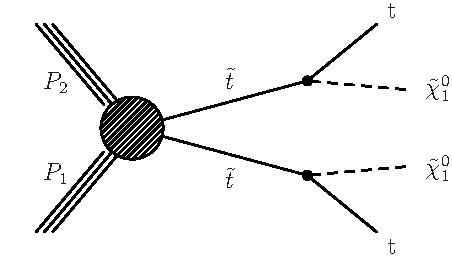
\includegraphics[width=0.40\textwidth]{sections/mc4/Introduction/figures/T2tt.pdf}\\
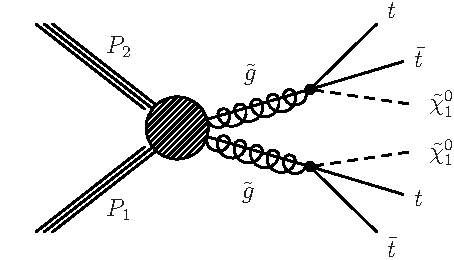
\includegraphics[width=0.33\textwidth]{sections/mc4/Introduction/figures/T1tttt_feynman.pdf}
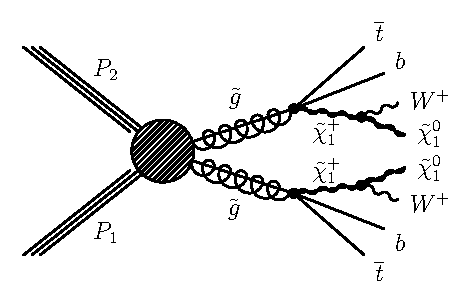
\includegraphics[width=0.33\textwidth]{sections/mc4/Introduction/figures/T1ttbb.pdf}\\
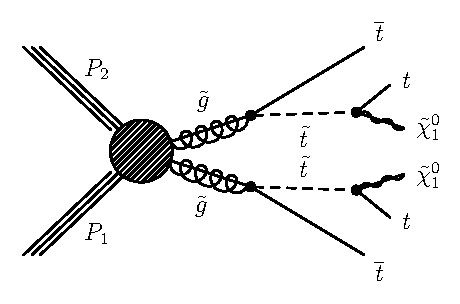
\includegraphics[width=0.33\textwidth]{sections/mc4/Introduction/figures/T5tttt.pdf}
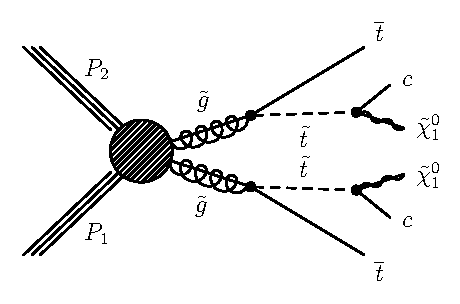
\includegraphics[width=0.33\textwidth]{sections/mc4/Introduction/figures/T5ttcc.pdf}\\
\caption{Signal models of interest in this search:
top squark pair production with the top squark decaying into a top quark and
neutralino (top),
and top squarks from cascade decays of gluinos (middle and bottom).
The SUSY simplified model topology shown at the top is referred to as T2tt,
the middle left model as T1tttt, middle right model as T1ttbb
the bottom left one as T5tttt and the bottom right one as T5ttcc.}
\label{fig:signal_diagrams}
\end{centering}
\end{figure}

The first step of the search is to design a search region with proper cuts. Since we are looking into all hadronic channels, we would veto the leptons and isolated tracks. The number of jets and \MET requirements are also needed to suppress the standard model background. A set of $\Delta\phi$ cuts between the \MET and several leading jets are also applied to reject QCD events. Moreover, since the signal final states have b-jets and top-jets, the numbers of b-jets and top-jets cuts are also added into the baseline selection. We use the official recommendation of b-jet tagger from CMS b-tagger working group. However, for the top-jet, we applied cut-based top jet identification in the 2015 analysis\cite{PhysRevD.96.012004}. In this 2016 analysis, we design a new top-jet identification algorithm to improve the analysis. Several working points are designed in top-jet tagger.

The next step is to determine the top-jet working point and optimize the search bins. We optimize the search bin definition for both medium and tight top-jet working point, and then choose the tight one because it is more sensitive for some signals.

Then, we need to estimate the backgrounds for all search bins. The major background is for TT-jets, W-jets and single top processes. The Z-jets, QCD, TTZ and other rare processes are not negligible, too.

Finally, we can set limit on the model parameters with the data yield, background estimation and targeting model yields. The interpretation is based on the simplified model\cite{Alwall:2008ag}.

